\documentclass{article}
\usepackage{blindtext}
\usepackage{graphicx}
\usepackage[utf8]{inputenc}
\graphicspath{ {Images/} }
\usepackage{biblatex}
\addbibresource{Test1.bib}

\title{Hot Chips}
\author{Gavin Barnett}
\date{\today}

\begin{document}
\maketitle
	\begin{figure}[h]
		\centering
		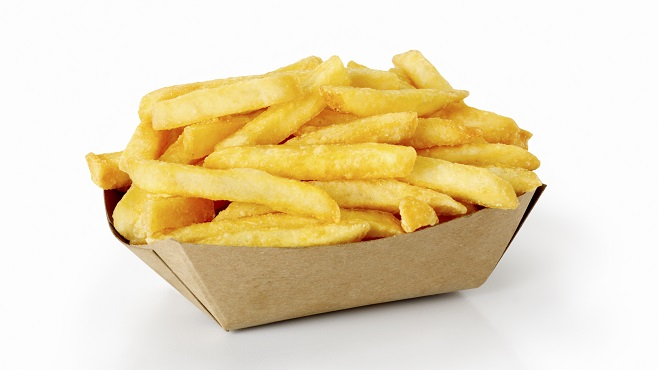
\includegraphics[scale=2.3]{Hot-chips-Getty}
		\caption{Hot-Chips}
	\end{figure}
\begin{abstract}
Random readings and rambling on the effects of high temperatures on electronic devices. 
Also getting use to using LaTeX.

\end{abstract}
\maketitle

\newpage

\tableofcontents

\newpage

\section{Introduction}

\newpage


\section{IC Packaging Considerations}
	\begin{figure}[h]
		\centering
		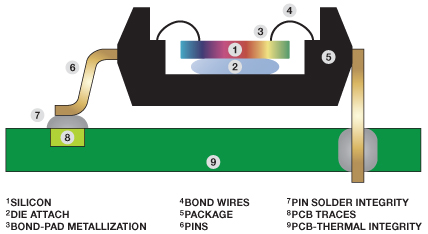
\includegraphics[scale=1]{Package_Breakdown}
		\caption{Packaging}
		\label{fig:packaging}
	\end{figure}
	
	
	\subsection{Silicon}
		\subsubsection{Crystalline structure failure}
		\subsubsection{Hot Carrier Injection (HCI)}
		\subsubsection{Negative Bias Temperature Instability (NBTI)}
	
	\subsection{Die Attach}
		\subsubsection{Coefficient of Thermal Expansion(CTE)}
	
	\subsection{Wire Bond/ Bond-Pad Metallization}
		\subsubsection{Inter-Metallic Compound (IMC) Growth}
		\subsubsection{Diffusion (Kirkendall Effect)}
		\subsubsection{Corrosion}
	
	\subsection{Package}
		\subsubsection{Glass-Transition Temperature (Tg)}
		\subsubsection{Coefficient of Thermal Expansion(CTE)}
		\subsubsection{Hermetic Ceramic Packages}
		\subsubsection{High-Temperature Multichip Modules}
	
	\subsection{Pins}
		\subsubsection{Through Hole}
		\subsection{Gull-Wing SMT}
		\subsubsection{BGA}
	
	\subsection{Pin Solder Integrity}
		% Ref: (http://www.logwell.com/tech/servtips/solder.html)
		% Ref2: (http://www.logwell.com/tech/app_notes/Temps.pdf)
		\subsubsection{Solder Alloys}
		\subsubsection{High Melting Point (HMP) alloys}
	
	\subsection{Printed Wiring Board (PWB)}
		\subsubsection{Glass Transition Temperature (Tg)}
		\subsubsection{De-lamination}
		\subsubsection{Moisture Absorption}

	\subsection{Printed Wiring Assembly (PWA)}
		\subsubsection{Tin-whiskers}
		\subsubsection{Flux residue}
		\subsubsection{Conformal Coating}

\newpage

\section{Passives}
	\subsection{Resistors}
	
	\subsection{Capacitors}
	
	\subsection{Inductors}
	
\newpage

\section{Fault Phenomenon}
	\subsection{Leakage Currents}
	In capacitors the "leakage current" is a small amount of current which flows across the dielectric material. This can also be expressed as a large shunt resistance known as "insulation resistance".
	
	\subsubsection{Dielectric Absorption Currents}
	This is the current required to align the dipoles with the dielectric.
	
	\subsubsection{Quantum Tunnel Effects}


\newpage

\printbibliography

\end{document}
